\documentclass[10pt,a4paper]{article}
\usepackage[margin=2.0cm]{geometry}
\usepackage[T1]{fontenc}
\usepackage{lmodern,microtype,graphicx,booktabs,amsmath,hyperref,caption,enumitem,url,seqsplit}
\captionsetup{font=small,labelfont=bf,skip=3pt}
\setlist{nosep,leftmargin=1.2em}
\setlength{\parskip}{3pt}\setlength{\parindent}{0pt}
\newcommand{\pt}{\,\text{pt}}
\title{\vspace{-1.2cm}\textbf{Selecting Reliable LLM Reasoning: Cross-Candidate and Arithmetic-Repair Evidence\\in a DeepSets Ensemble for Choosing 1 of 4 Qwen3-0.6B GSM8K Solutions}\vspace{-0.3cm}}
\author{Name / Student ID \quad (DASE7506 MP2)}
\date{}
\begin{document}
\maketitle\vspace{-0.8cm}
\begin{abstract}\small
For each GSM8K question we must pick one of four Qwen3-0.6B candidate solutions; the score is the selection accuracy of the chosen final answer. Majority vote (ties to the longest trace) is a strong baseline. We build a learned selector that scores each candidate from hand-made answer/format/arithmetic features, group-relative (within-question) normalisation, and the full 1024-d supplied embedding, trained with a listwise loss $-\log\sum_{\text{correct}}p$ and decoded by summing probability over identical parsed answers. Our first neural model (v2, 5-member DeepSets) reached 80.5\% hard-group accuracy in 5-fold train-only CV and 81.58\% on test. Two families of \emph{cross-candidate text evidence} then gave the only robust gains: (v3) whether the other candidates' final answers occur inside a candidate's reasoning and vice versa (+1.4\pt CV), and (v4) \emph{arithmetic repair}, i.e.\ recomputing each trace with earlier slips corrected and checking whether the corrected answer lands on another candidate's answer (+1.2\pt CV; idea adapted from another student's public repository). The final v4 model, a 10-member DeepSets ensemble (8.9\,MiB, numpy-only inference, 2--3\,s), reaches 83.1\% CV-hard, 87.0\% val-hard, 94.24\% val-all and \textbf{82.66\% (386/467) on test}. Ablations show that the embedding (not length or format shortcuts) carries most of the signal, that comparing candidates helps through their \emph{text} (shared intermediate values, corrected arithmetic) rather than through learned interaction layers, that the model is well calibrated, and that larger models, relational layers and stacking do not pay off. The test bank was scored once for each of three frozen versions (v2, v3, v4); we report all three.
\end{abstract}

\section{Task and data}
Data: 4755 train, 798 validation and 467 test questions, four candidates each, with fixed embeddings of shape $[N,4,1024]$. Every group contains at least one correct answer (an oracle selector reaches 100\%); mean per-candidate accuracy is about 0.755. About 5\% of candidates have no parseable answer (5.9\% on test).

\textbf{Hard groups.} A group is \emph{hard} if its four candidates contain at least two distinct valid parsed answers, i.e.\ selection is non-trivial. Test consists \emph{only} of hard groups (467); train has 2114 hard groups and validation 355. Hard groups always contain between one and three correct candidates. Because validation also contains easy groups (where any choice is right) its overall accuracy is inflated, so \textbf{val-hard is the test-like metric}; we report val-all only for completeness. Hard-group accuracy of simple rules on validation: first candidate 54.9, random 51.1, vote with ties to lowest index 69.0, vote with ties to the longest 70.7. One validation hard group is 0.28\pt; a Wilson 95\% interval for a single accuracy is about $\pm4.5$\pt, so differences below roughly 3\pt are not resolvable on validation alone.

\section{Methods}
\textbf{Vote baseline.} Cluster candidates by parsed answer (the fixed \texttt{common.parse\_answer}), pick the most frequent answer, break ties toward the longest trace (longest wins ties 50\% of the time vs.\ 27\% for shortest on train, so short traces are often wrong).

\textbf{Features (shared by LR and NN).} 37 hand features per candidate: vote count/share/number of distinct answers/is-top flags; answer-level (parse validity, integer, negative, magnitude, rank among answers, answer equals a number in the question); surface/format (seven length features, \verb|\boxed|/\verb|####|/placeholder flags, truncation, number of lines, ``final answer'' count, hedging words); reasoning content (a shallow arithmetic checker on equations in the trace, question-number coverage, answer repeated in the body, cluster-level arithmetic statistics); plus cross-candidate cosines of embeddings (to the same-answer and different-answer candidates). All features are also entered \emph{group-relative} (minus the group mean), so a candidate is judged against its three siblings.

\textbf{v1: logistic regression.} Hand+cross features plus a 64-d PCA of the embedding, group-relative, one logistic regression ($C=10$, trained on hard groups), decoded by cluster-sum (sum of candidate probabilities per distinct answer, take argmax). 275\,KB.

\textbf{v2: DeepSets ensemble.} A per-candidate encoder consumes the standardised features and the full standardised 1024-d embedding (input dropout 0.3, first layer $1024\to128$, two layers, $H=128$, dropout 0.3). A DeepSets block concatenates $[h,\;h-\bar h,\;\bar h,\;\text{mean of }h\text{ over same-answer candidates}]$ before the score head. Training is listwise: $\mathcal L=-\log\sum_{c\in\text{correct}}\mathrm{softmax}(s)_c$, so credit goes to \emph{any} correct candidate (matching the scorer, which accepts any correct answer). AdamW (lr $10^{-3}$, wd 0.05, batch 64, $\le60$ epochs), training on hard groups only, early stopping (patience 8) on a 12\% train-internal holdout (stops at epoch 2--9: the model overfits quickly, regularisation is crucial). Five members (seeds 0--4) are averaged in probability space; decode is the cluster-sum above. Inference is pure numpy (matches torch to $1.8\times10^{-7}$), no pickle; torch is only needed for training.

\textbf{v3: cross-candidate text features.} A probe of v2's out-of-fold errors on train showed a signal that per-candidate embeddings cannot see: a wrong candidate often stops early at an intermediate value of a correct chain. If \emph{every} other distinct answer occurs as a number inside candidate $i$'s reasoning, $i$ is correct 75\% of the time (n=1353, base 50\%); if $i$'s answer occurs inside every other-answer trace, only 40\% (n=1428). v3 adds 15 such features (\texttt{features\_v3.py}): fraction/any of other-answer traces containing my answer and vice versa, the latest position at which another answer occurs in my trace, first position of my own answer, number-set Jaccard to same-/different-answer traces, fraction of my numbers grounded in the question or in other traces, question-number coverage including number words, cluster means. Same DeepSets model; ensemble size raised to K=10 because v3 kept gaining from K=5 to 10 (+0.5 CV) where v2 did not.

\textbf{v4 (final): arithmetic repair.} 13 more features (\texttt{features\_repair.py}), an independent implementation of an idea from another student's public MP2 repository (github.com/Devin-Lo1/dase-7506-mp2, \texttt{repair90.py}; see Section~9). LaTeX is normalised to plain arithmetic (\verb|\frac|, \verb|\times|, \%, markdown bold), and every \verb|lhs = rhs| in the trace is extracted (nearest arithmetic run on each side of each \verb|=|) and evaluated with a restricted AST walker (numbers and $+-\times\div$ only; text is never executed). Walking the equations in order, each lhs is recomputed with earlier corrections substituted at every sub-result, so one slip propagates; each mismatch records (written value $\to$ corrected value). If the final answer is a written value that was corrected, the corrected value is the trace's \emph{repaired answer}, i.e.\ what the same method gives with correct arithmetic. Features: equation/error/repair counts, propagated errors, a final-answer-repaired flag, \emph{support} (number of other traces whose repaired answer equals my answer), whether my repaired answer equals another candidate's answer, and the vote share after every trace votes for its repaired answer. On train, support marks 83\% correct candidates (n=334, base 49\%) and ``my repaired answer equals another candidate's'' 22\% (n=243); the repaired flag alone is uninformative (49\%) because the extractor also produces spurious repairs, so the value is in the cross-candidate matches. Everything else is unchanged from v3: K=10 (seeds 0--9), sum decode, train split only.

\section{Experimental protocol}
\begin{itemize}
\item \textbf{Train-only fitting.} Every parameter, PCA, standardiser and early-stopping holdout is fit on the train split only; we do \emph{not} refit on train+val.
\item \textbf{Honest selection estimate: 5-fold train-CV} (group folds, seed 0) scoring hard held-out groups; 2114 hard groups pooled, fold std 1.5--2.5\pt, pooled standard error about 0.9\pt. Final design choices (C, interaction type, K, features) were made on CV, picking the simplest config within CV noise of the best.
\item \textbf{Validation as secondary.} Some variants were also compared on val-hard, so val numbers carry selection bias.
\item \textbf{Test use.} The official test bank was scored once for each of three frozen versions: v2 (2026-10-21), v3 and v4 (2026-10-28). Each version was frozen on CV and validation before its test run, and no test result was used to tune features, hyperparameters, K or decoding. The sequence is not test-blind, however: v4 was developed after v3's lower test score was known and after seeing another student's higher score and method, so the v4 test number carries a small amount of sequential selection. We report all three test scores.
\item Seeds: v2 members 0--4, v3/v4 members 0--9 (init and holdout split seeded identically); v2 ablations use val 3 seeds (0--2) and CV 2 seeds (0,1); v3/v4 variants use 5 or 10 seeds on both CV and val. Wilson 95\% CIs are reported for single accuracies.
\end{itemize}

\section{Results}
\begin{table}[h]\centering\small
\caption{Main results (\%). Val-hard n=355, CV-hard n=2114 (10-seed ensembles for v3/v4), test n=467 (all hard). Time = fresh \texttt{predict.py}+scorer on validation, 4 threads, local 2-core EPYC. Test was run once per frozen version (v2, v3, v4).}
\setlength{\tabcolsep}{4pt}\begin{tabular}{lcccccrr}\toprule
Method & val-all & val-hard [95\% CI] & CV-hard & test & time (s) & assets\\\midrule
Majority vote (tie$\to$longest) & 86.97 & 70.7 [65.8, 75.2] & 69.9 & -- & 0.38 & 0\\
v1 LR (hand+cross+PCA64) & 91.10 & 80.0 [75.5, 83.8] & 77.3 & -- & 1.07 & 269\,KiB\\
v2 DeepSets, K=1 & 92.73 & 83.7 [79.5, 87.1] & 80.0 & -- & 1.11 & 885\,KiB\\
v2 DeepSets, K=5 & 93.23 & 84.8 [80.7, 88.2] & 80.4 & 81.58 & 1.38 & 4424\,KiB\\
v3 = v2 + cross-candidate text, K=10 & 93.48 & 85.4 [81.3, 88.7] & 81.9 & 80.73 & 2.26 & 9003\,KiB\\
\textbf{v4 = v3 + arithmetic repair, K=10 (final)} & \textbf{94.24} & \textbf{87.0} [83.1, 90.1] & \textbf{83.1} & \textbf{82.66} & 3.09 & 9135\,KiB\\\bottomrule
\end{tabular}
\end{table}
The final test score is 386/467 = 82.66\% (Wilson 95\% CI [79.0, 85.8]); predict+score took 2.1--2.4\,s wall and 95\,MB on test. The CV figure (83.1, fold std 1.5) is the honest selection estimate; val-hard (87.0) is optimistic because variants were also compared on it. v3 is instructive: it improved CV by 1.4\pt and val by 0.6\pt but lost 4 test groups to v2 (80.73 vs 81.58). With a test CI of about $\pm3.5$\pt neither difference is resolvable; we did not switch versions on that basis. v4 improved all three (CV +2.6, val-hard +2.2, test +1.1 over v2). Against vote on val-hard, v4 fixes 70 groups and breaks 12 (v2: 61/11). v2 single-model K differences are far inside noise.

\section{Research questions}
\textbf{RQ1: Does reading the reasoning help beyond voting?}
\emph{Hypothesis:} voting already captures most signal; text content helps modestly through arithmetic checks, and the embedding encodes something about reasoning quality.
Cumulative information ablation (Fig.~\ref{fig:info}; same NN architecture, features zeroed, val 3 seeds / CV 2 seeds): vote only 67.9/66.6 (val-hard/CV-hard), +answer-level 72.6/71.9, +surface/format 76.7/73.1, +hand reasoning content 77.9/75.2, +embeddings 83.6/79.8. Embeddings alone (no hand features, no vote) reach 79.2/77.1, more than all hand features together. Leaving one group out of the full model: removing answer-level hurts most (79.8/78.4), removing reasoning-content costs 0.5 val / 1.3 CV, removing surface/format 1.3 val and +0.3 CV (nil).
\emph{Conclusion:} partly confirmed. Reading helps, mainly via the embedding (+5.7 val/+4.6 CV over hand features); the v1 hand arithmetic checker adds little because it rarely fires (about two equations per candidate), which also explains why the v2 verifier features (RQ5) failed. The repair features of v4 show that \emph{reading the arithmetic properly} does help: with LaTeX normalisation and nearest-run extraction they parse most equations, and the gain is concentrated exactly where expected. On the 186 train hard groups in which some trace's repaired answer supports another candidate, CV accuracy rises from 78.5 (v3) to 88.2 (v4), versus 82.2$\to$82.6 on the rest. A post-hoc check with the test labels (not used for any decision) found the same pattern: 7.5\% of test groups contain a ``right method, arithmetic slip'' candidate, and v2 solved only 74\% of those groups versus 82\% elsewhere.

\begin{figure}[t]\centering
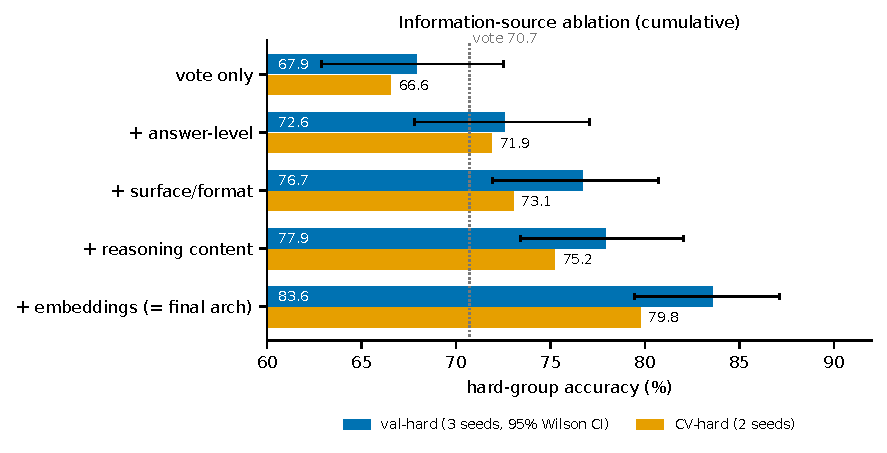
\includegraphics[width=0.62\linewidth]{figures/fig_info_ablation.pdf}\hfill
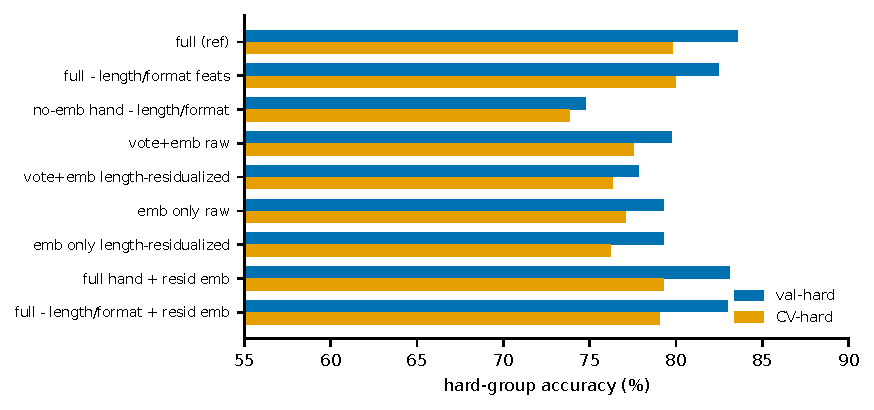
\includegraphics[width=0.36\linewidth]{figures/fig_shortcut.pdf}
\caption{Left: cumulative information ablation. Right: shortcut ablations (bars: val-hard, CV-hard) for RQ2. Both on the v2 model.}\label{fig:info}
\end{figure}

\textbf{RQ2: What makes a wrong answer convincing; does the model use shortcuts?}
\emph{Hypothesis:} length and format are shortcuts (long, boxed traces look right); the embedding mostly encodes length/format, so it would collapse once length is regressed out.
Evidence (Fig.~\ref{fig:info}, right; val-hard/CV-hard): removing length/format features from the full model gives 82.4/80.0 (vs 83.6/79.8), i.e.\ no loss with the embedding present, but without the embedding it drops (74.7/73.8 vs 77.9/75.2 hand-only). Regressing the embedding on length/format ($R^2=0.055$) and using the residual keeps accuracy (full 83.1/79.3; emb-only 79.2/76.2 vs 79.2/77.1). Stratifying val-hard by which trace is longest: when the longest is correct and the shortest wrong (n=141) the model gets 91.5; longest wrong/shortest correct (n=76) 84.2 while picking the longest only 7\%; both extremes wrong (n=80) 63.7. It picks the longest in 41\% and shortest in 10\% of groups (always-longest 56.1, always-shortest 37.7). Wrong picks are only slightly longer than the alternatives (log-ratio +0.061 vs +0.117 for right picks).
\emph{Conclusion:} rejected as a main driver. Length is a usable weak cue (the vote tie-break uses it) but the learned model does not depend on it. What makes wrong answers convincing is agreement: in 50\% of errors the plurality answer is wrong, i.e.\ a shared misreading of the question (Section~6).

\textbf{RQ3: Can a candidate be judged on its own, or is cross-candidate comparison needed?}
\emph{Hypothesis:} comparison matters because correctness is relative within a group.
Evidence (val-hard 3 seeds / CV-hard): strict per-candidate scoring (all group-relative, vote, cluster and cosine features removed, argmax decode) 83.1/78.7, versus the full no-interaction model 83.6/79.6 and DeepSets 83.6/79.8 (argmax: 83.2/79.0). Single-model attention is worse and noisier (82.2$\pm$1.5). Cluster-sum decoding adds 0.6--1.3\pt CV (79.8 vs 79.0 full; 80.0 vs 78.7 without cross-candidate features), the only reliable cross-candidate gain.
\emph{Conclusion (v2):} mostly rejected: the per-candidate score from the full embedding is almost as good, and cross-candidate information is worth about +1\pt CV, via answer-level aggregation. The explicit DeepSets interaction itself adds $\approx0$ (differences $\le0.3$\pt, within noise).

\emph{Revised by v3/v4:} comparison \emph{does} matter, but through the candidates' \emph{text}, not through learned interaction over embeddings. Features that ask whether one trace contains another's final answer (v3, +1.4\pt CV) or whether one trace's corrected arithmetic produces another's answer (v4, +1.2\pt CV) are the two largest gains after the embedding itself. With these features present, the interaction layer still adds nothing: per-candidate MLP 81.5 vs DeepSets 81.4 (K=5 CV). A relational block with learned messages over pair features (answer-in-reasoning, number-set overlap, embedding cosine, magnitude ratio, where the number chains diverge, $|e_i-e_j|$) gave 81.5--81.9 at K=5 and 81.8 at K=10, the same as v3's 81.9. Cross-candidate evidence is best computed explicitly, not learned from 2114 groups.

\textbf{RQ4: Does the model know when it is uncertain?}
\emph{Hypothesis:} the cluster probability mass is a usable confidence; disagreement with the vote signals risk.
Evidence (Fig.~\ref{fig:unc}): out-of-fold CV ECE 0.016 (accuracy 80.5, mean confidence 80.7), val-hard ECE 0.039 (84.8 vs 82.5), Brier 0.111. Selective accuracy by coverage (val-hard / CV-hard): 50\% coverage 96.1/94.9, 70\% 93.2/90.2, 90\% 87.2/84.1, 100\% 84.8/80.5. Margin between top two answer clusters: below 0.1 gives 59.1\% (n=22), 0.9--1.0 gives 100\% (n=130). When final model, LR and vote all agree accuracy is 88.1 (n=269) against 74.4 for the other 86 groups.
\emph{Conclusion:} confirmed. Probabilities are well calibrated on CV and slightly under-confident on val; abstaining on the least confident half would give $\sim$95\% accuracy, a useful property although the task requires an answer for every question. The final v4 model behaves the same (out-of-fold CV ECE 0.028: accuracy 83.1, mean confidence 82.5; val-hard ECE 0.041; selective CV accuracy 95.5/91.2/86.3/83.1 at 50/70/90/100\% coverage). Figures show v2.

\begin{figure}[t]\centering
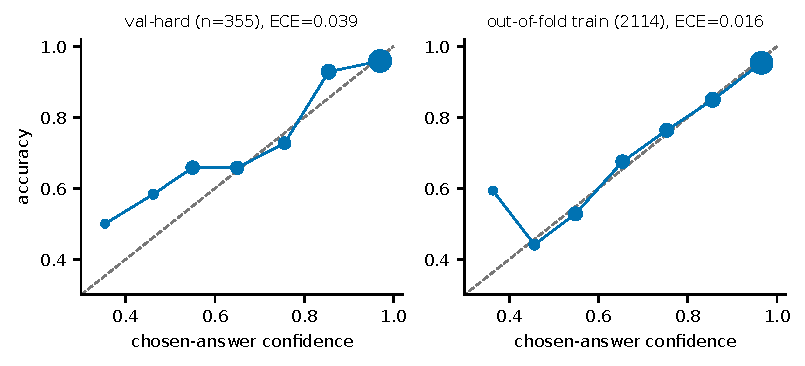
\includegraphics[width=0.48\linewidth]{figures/fig_calibration.pdf}\hfill
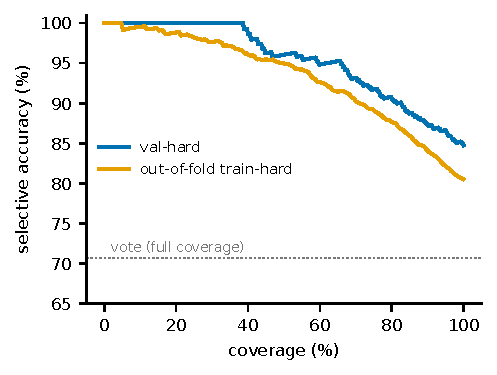
\includegraphics[width=0.48\linewidth]{figures/fig_selective.pdf}
\caption{Calibration (left) and selective accuracy versus coverage (right) of the v2 K=5 ensemble (v4 figures in RQ4 text).}\label{fig:unc}
\end{figure}

\textbf{RQ5: Does more computation pay off?}
\emph{Hypothesis:} more members and richer verification give diminishing returns.
Evidence (Fig.~\ref{fig:comp}, Table 1): CV-hard for K=1/3/5/10 is 79.96/80.24/80.45/80.45, wall 1.11/1.24/1.35/1.68\,s (about 0.06\,s per member, 0.9\,MiB each); val-all K=10 is 92.86. Training is cheap: features 4.0\,s, LR fit 1.5\,s, NN 4.9\,s per member (24.7\,s for K=5). Moving from vote to LR costs +0.7\,s for +7.4\pt CV; LR to a single NN costs +0.04\,s for +2.7; K=1 to K=5 costs +0.27\,s for +0.5 (inside noise). A second, more expensive verifier family (v2: chained/unit/percentage arithmetic, wrong-step fraction, last-equation-equals-answer, plausibility vs question numbers) was a \emph{negative} result: CV $-0.55$ for LR, $-0.1$ to $+0.25$ for NN, so it was discarded. Likewise self-attention across candidates and HGB trees (79.2 hard, no gain over LR) were dead ends.
\emph{Conclusion (v2):} confirmed. The embedding with a small regularised network is the efficient frontier; K=5 is a conservative choice and K=3 would do equally well.

\emph{v3/v4 search} (5- or 10-seed CV-hard; full table in \texttt{code/method/results\_v3.md}). With v3 features, every extra-computation variant stayed within noise:
\begin{itemize}
\item width $H$=64/256: 81.1/81.2;
\item stronger dropout or weight decay, lower learning rate: 81.0--81.4;
\item relational pair-message block and its variants: 81.5--81.9;
\item pooling v3 and relational ensembles (20 members, over the 16\,MiB limit): 82.1;
\item a TF-IDF character n-gram text model (71.1 alone, +0.2 blended);
\item gradient-boosted stacking on out-of-fold scores (+0.1 to +0.5 depending on the decode rule, not robust).
\end{itemize}
What paid off were cheap \emph{features}. v3 costs +0.9\,s at inference for +1.4\pt CV, and repair costs +0.8\,s for +1.2\pt; both are dominated by Python regex/AST parsing. Ensemble size mattered more for v3/v4 than for v2 (v4 K=1/5/10: 81.4/82.4/83.1), so we doubled K at 0.9\,MiB and about 0.06\,s per member. Mean pooling of answer clusters (used in the repository the repair idea came from) cost 1.7\pt CV against our probability-sum decode and was rejected.

\begin{figure}[t]\centering
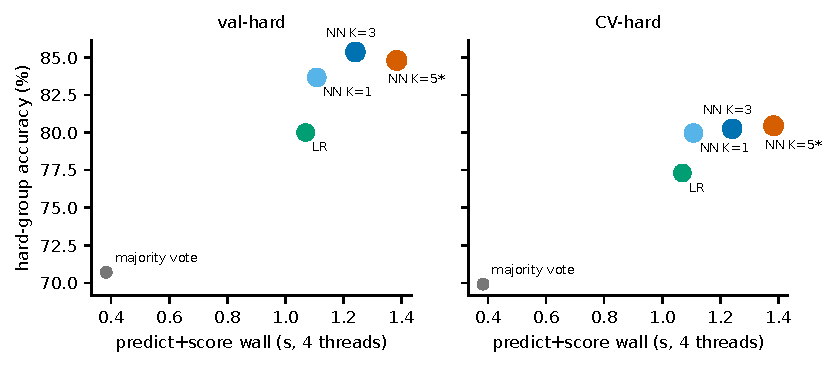
\includegraphics[width=0.62\linewidth]{figures/fig_compute.pdf}
\caption{Accuracy versus inference wall time (val-hard left, CV-hard right). Star: v2 K=5 (v2 analysis; v3/v4 costs in the text and Table 1).}\label{fig:comp}
\end{figure}

\section{Failure analysis}
\textbf{Final v4.} Of 355 val-hard groups v4 errs on 46. By vote structure: plurality answer wrong 22, 2--2 tie lost 14, all four answers distinct 7, overrode a correct plurality 3. Repair removed most of v2's ``correct trace with a slip'' losses, so the remaining errors are dominated by shared misreadings (below), which no candidate-only evidence can resolve.

\textbf{v2 analysis} (details below are for the v2 model). Of 355 val-hard groups v2 errs on 54. Automatic categories by vote structure: plurality answer wrong 27, all four answers distinct 14, 2--2 tie lost 6, picked a non-plurality answer 4, overrode a correct plurality 3. Accuracy by vote pattern (right/n): 3--1: 138/151, 2--1--1: 69/88, 2--2: 28/34, 1--1--1--1: 15/20, 1--1--1: 14/20. Eleven errors involve a group with an unparseable trace, and in four of those the unparseable trace visibly contains the gold answer (scorer-format loss). A manual reading of 20 errors (every second error, bank order) gives: shared misreading by $\ge2$ traces 9, hard problem with no vote signal 5, coin-flip 2--2 tie 2, correct trace lost to format 2, confident singleton overriding the correct plurality 2.
\begin{itemize}
\item \emph{Group 586, shared misreading.} Three traces compute the absent students as $250-70=180$ (\verb|\boxed{180}|); the single correct trace (\verb|250 - 140 - 70 = 40|) gets $p=0.06$. No feature that sees only candidates can tell which reading is right.
\item \emph{Group 444, format loss.} The correct answer 40 appears only in traces ending in ``Final Answer: **40 meters**'' with no \verb|####|/\verb|\boxed|, hence unparseable; the model picks 45 (\verb|\boxed{45}|) with $p=0.94$.
\end{itemize}
Where it succeeds: against vote it wins 61 and loses 11; on groups where the top count is tied (n=88) it gets 77.3 vs 50.0 for vote.

\section{Limitations}
\begin{itemize}
\item \textbf{Selection bias.} Variants were compared on val-hard (355 groups), so those numbers (87.0, 94.24 for v4) are optimistic; CV (83.1) is the honest selection estimate. The test bank was scored for three successive frozen versions; each run was blind to the next version's design choices, but the decision to keep improving after v3, and the source of the v4 idea, were influenced by test-level outcomes (ours and another student's). The v4 test score (82.66) should therefore be read as slightly optimistic as well.
\item \textbf{Repair extractor noise.} The equation extractor is heuristic: it misses equations in prose (``24 inches plus 16 inches is 40''), and produces spurious ``repairs'' (the repaired-flag alone has no predictive value). The model relies on the cross-candidate matches, which are much less noisy.
\item \textbf{Noise.} One group is 0.28\pt on val-hard and 0.05\pt on pooled CV; CIs are about $\pm4.5$\pt on val and $\pm3.5$\pt on test. K and interaction comparisons are not resolvable; ablation deltas under about 1\pt (CV) should be read as zero. CV std over seeds is 0.2--0.6, over folds 1.5--2.5.
\item \textbf{Scorer checks final answers only.} The selector is rewarded for the final number, not for valid reasoning; a trace with wrong steps and a lucky right answer counts as correct, and we cannot make claims about reasoning validity.
\item \textbf{Embedding opacity.} The main gain comes from a 1024-d representation we cannot interpret; our shortcut checks (length/format residualisation, $R^2=0.055$) rule out only the cues we thought of, and the gain may reflect candidate-generation style specific to Qwen3-0.6B/GSM8K. Generalisation to another generator or domain is untested; test texts are somewhat longer than train.
\item Hard-group training is tuned to a test of hard groups only; a bank with many easy groups is handled by the same code but was not tuned for.
\end{itemize}

\section{Resource use and reproducibility}
\textbf{Hardware/software.} Local machine AMD EPYC 7A23 (2 cores available), no GPU, Python 3.12.3, numpy 2.5.3, scikit-learn 1.9.1, scipy 1.18.1 for inference/features; torch 2.14.1 (CPU) only for training; matplotlib 3.11.2 for figures. \textbf{Training cost:} base features 4.0\,s, v3 features 2.3\,s, repair features 6.5\,s (train+val), about 4--5\,s per NN member. Exporting the final 10-member checkpoint (\texttt{python method/exp3.py export K=10 rep=1 out=checkpoint}) takes about 1\,min wall on this machine. Each 5-fold $\times$ 10-seed CV run of a v3/v4 variant takes about 4\,min; all v3/v4 experiments together took about 1.5\,h of CPU. No GPU or remote machine was used for any reported result. \textbf{Inference:} fresh \texttt{predict.py} plus scorer with 4 threads: 3.1\,s on validation (798 groups; 125\,MB RSS) and 2.1--2.4\,s on test (95\,MB) on the local EPYC 7A23 machine. The eligibility limit (30\,s on the reference Xeon Platinum 8457C) is not measured on that CPU; we have about a 10$\times$ margin locally. \textbf{Assets:} \texttt{code/checkpoint/nn.npz} 9{,}351{,}582\,B (sha256 \texttt{\seqsplit{8a1c1006060db7301901b8b20bea9f9957d074173b5b2e9a2c15b046bde77841}}) and \texttt{config.json} 2{,}463\,B (sha256 \texttt{\seqsplit{3f7cd767a02f2efbd98943be4e90e6ae0a14bfb2223678581db4f6e1ff398df4}}), 8.92\,MiB in total (limit 16\,MiB). Re-running the training command into a scratch directory reproduces both files bit-for-bit (identical sha256). Earlier versions are kept for ablation (\texttt{checkpoint\_v3/}, \texttt{checkpoint\_v2/}, \texttt{checkpoint\_lr/}). All commands, seeds and result files are listed in the top-level \texttt{README.md}; official JSONs are in \texttt{code/results/} (\texttt{v2-*}, \texttt{v3-*} for earlier versions).

\section{AI use and reuse disclosure}
The code (features, models, training, numpy inference, analysis scripts), the experiments and the first draft of this report were produced substantially by Claude Code (Anthropic) AI agents working under the student's direction; the student specified the task and constraints, reviewed results and is responsible for the submission. No external data, pretrained weights or additional datasets were used; no LLM is called at inference. \textbf{Reused idea:} the arithmetic-repair features (v4) adapt the idea of \texttt{repair90.py} in another student's public MP2 repository, \url{https://github.com/Devin-Lo1/dase-7506-mp2}. An AI agent read that repository statically (its code was not executed), and our \texttt{features\_repair.py} is an independent implementation. The same repository prompted our mean-versus-sum pooling check, which we rejected. Other reused material: the supplied course package (data, parser, scorer, \texttt{predict.py}), numpy, scikit-learn, scipy, PyTorch and matplotlib. Data: questions and references derive from GSM8K (MIT licence, Cobbe et al., OpenAI); candidate solutions and embeddings were prepared with Qwen3-0.6B (Qwen team, Alibaba) and supplied by the course; the licence and attribution files are kept in \texttt{code/data/}.
\end{document}
